\documentclass[tikz,border=12pt]{standalone}
\usepackage[T1]{fontenc}
\usepackage{mathpazo}
\usepackage{amsmath,amssymb}
\usetikzlibrary{arrows.meta, positioning, calc, decorations.pathreplacing}

\definecolor{stblue}{HTML}{7B97AD}
\definecolor{rwgold}{HTML}{B8995E}
\definecolor{sage}{HTML}{7A9A7E}
\definecolor{dkbrown}{HTML}{3D3530}
\definecolor{wmgray}{HTML}{7B7067}
\definecolor{cream}{HTML}{F9F6F0}
\definecolor{border}{HTML}{D4C9B8}
\definecolor{terracotta}{HTML}{C47A6A}

\begin{document}
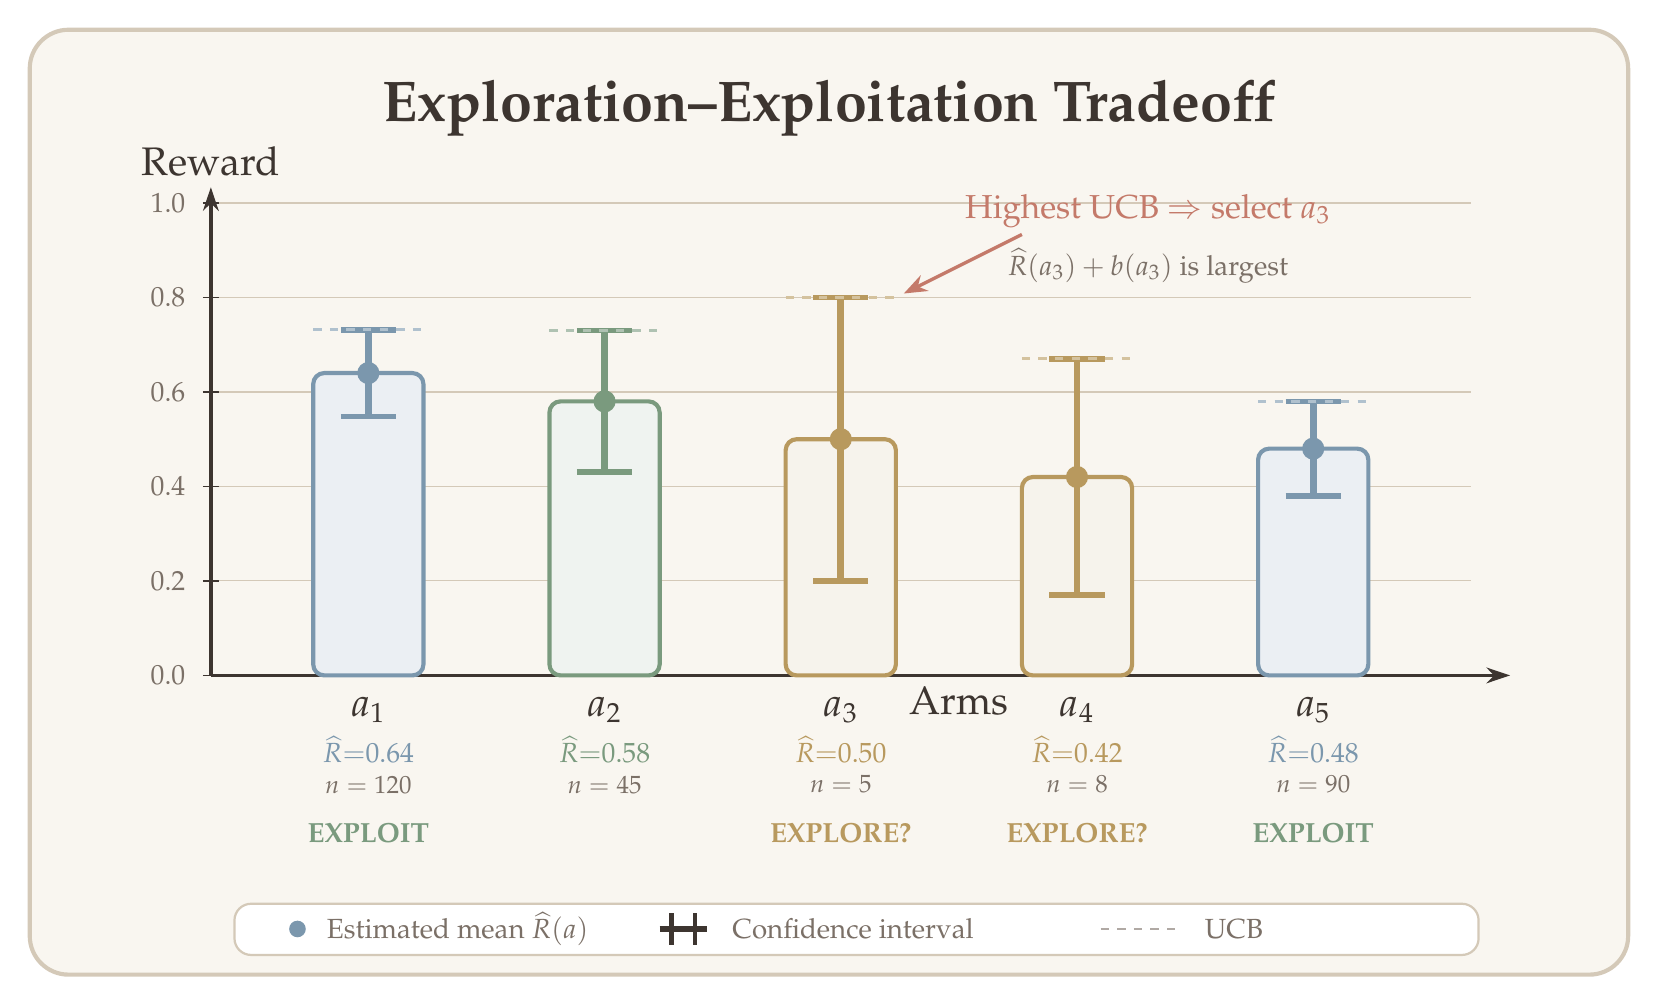
\begin{tikzpicture}[
  >={Stealth[length=3mm, width=2mm]},
]

% Background
\fill[cream, rounded corners=14pt] (-1.8,-3.8) rectangle (18.5,8.2);
\draw[border, rounded corners=14pt, line width=1.5pt] (-1.8,-3.8) rectangle (18.5,8.2);

% Title
\node[font=\huge\bfseries, text=dkbrown] at (8.35,7.2)
  {Exploration--Exploitation Tradeoff};

% Axes
\draw[dkbrown, line width=1.2pt, ->] (0.5,0) -- (17,0)
  node[below, font=\Large, text=dkbrown, xshift=-7cm] {Arms};
\draw[dkbrown, line width=1.2pt, ->] (0.5,0) -- (0.5,6.2)
  node[above, font=\Large, text=dkbrown] {Reward};

% Y-axis ticks
\foreach \y/\val in {0/0.0, 1.2/0.2, 2.4/0.4, 3.6/0.6, 4.8/0.8, 6.0/1.0} {
  \draw[dkbrown, line width=0.6pt] (0.4,\y) -- (0.6,\y);
  \node[left, font=\normalsize, text=wmgray] at (0.3,\y) {\val};
}

% Grid lines
\foreach \y in {1.2, 2.4, 3.6, 4.8, 6.0} {
  \draw[border, line width=0.4pt] (0.6,\y) -- (16.5,\y);
}

% =============================================
% Arm definitions: x-pos, mean, CI-half, color, name, n-count, label
% =============================================

% Arm 1: well-explored (narrow CI)
\def\axA{2.5}
\def\meanA{3.84} % 0.64 * 6
\def\ciA{0.55}   % narrow
\fill[stblue!15, rounded corners=4pt] (\axA-0.7, 0) rectangle (\axA+0.7, \meanA);
\draw[stblue, line width=1.5pt, rounded corners=4pt] (\axA-0.7, 0) rectangle (\axA+0.7, \meanA);
% CI
\draw[stblue, line width=2.5pt] (\axA, \meanA-\ciA) -- (\axA, \meanA+\ciA);
\draw[stblue, line width=2pt] (\axA-0.35, \meanA-\ciA) -- (\axA+0.35, \meanA-\ciA);
\draw[stblue, line width=2pt] (\axA-0.35, \meanA+\ciA) -- (\axA+0.35, \meanA+\ciA);
% UCB dashed line
\draw[stblue!60, line width=1pt, dashed] (\axA-0.7, \meanA+\ciA) -- (\axA+0.7, \meanA+\ciA);
% Mean dot
\fill[stblue] (\axA, \meanA) circle (4pt);
% Labels
\node[below, font=\Large\bfseries, text=dkbrown] at (\axA, -0.15) {$a_1$};
\node[below, font=\normalsize, text=stblue] at (\axA, -0.65) {$\widehat{R}{=}0.64$};
\node[below, font=\small, text=wmgray] at (\axA, -1.15) {$n=120$};
\node[below, font=\normalsize\bfseries, text=sage] at (\axA, -1.75) {EXPLOIT};

% Arm 2: moderately explored
\def\axB{5.5}
\def\meanB{3.48} % 0.58 * 6
\def\ciB{0.9}
\fill[sage!12, rounded corners=4pt] (\axB-0.7, 0) rectangle (\axB+0.7, \meanB);
\draw[sage, line width=1.5pt, rounded corners=4pt] (\axB-0.7, 0) rectangle (\axB+0.7, \meanB);
\draw[sage, line width=2.5pt] (\axB, \meanB-\ciB) -- (\axB, \meanB+\ciB);
\draw[sage, line width=2pt] (\axB-0.35, \meanB-\ciB) -- (\axB+0.35, \meanB-\ciB);
\draw[sage, line width=2pt] (\axB-0.35, \meanB+\ciB) -- (\axB+0.35, \meanB+\ciB);
\draw[sage!60, line width=1pt, dashed] (\axB-0.7, \meanB+\ciB) -- (\axB+0.7, \meanB+\ciB);
\fill[sage] (\axB, \meanB) circle (4pt);
\node[below, font=\Large\bfseries, text=dkbrown] at (\axB, -0.15) {$a_2$};
\node[below, font=\normalsize, text=sage] at (\axB, -0.65) {$\widehat{R}{=}0.58$};
\node[below, font=\small, text=wmgray] at (\axB, -1.15) {$n=45$};

% Arm 3: poorly explored (wide CI)
\def\axC{8.5}
\def\meanC{3.0} % 0.50 * 6
\def\ciC{1.8}
\fill[rwgold!12, rounded corners=4pt] (\axC-0.7, 0) rectangle (\axC+0.7, \meanC);
\draw[rwgold, line width=1.5pt, rounded corners=4pt] (\axC-0.7, 0) rectangle (\axC+0.7, \meanC);
\draw[rwgold, line width=2.5pt] (\axC, \meanC-\ciC) -- (\axC, \meanC+\ciC);
\draw[rwgold, line width=2pt] (\axC-0.35, \meanC-\ciC) -- (\axC+0.35, \meanC-\ciC);
\draw[rwgold, line width=2pt] (\axC-0.35, \meanC+\ciC) -- (\axC+0.35, \meanC+\ciC);
\draw[rwgold!60, line width=1pt, dashed] (\axC-0.7, \meanC+\ciC) -- (\axC+0.7, \meanC+\ciC);
\fill[rwgold] (\axC, \meanC) circle (4pt);
\node[below, font=\Large\bfseries, text=dkbrown] at (\axC, -0.15) {$a_3$};
\node[below, font=\normalsize, text=rwgold] at (\axC, -0.65) {$\widehat{R}{=}0.50$};
\node[below, font=\small, text=wmgray] at (\axC, -1.15) {$n=5$};
\node[below, font=\normalsize\bfseries, text=rwgold] at (\axC, -1.75) {EXPLORE?};

% Arm 4: poorly explored (wide CI)
\def\axD{11.5}
\def\meanD{2.52} % 0.42 * 6
\def\ciD{1.5}
\fill[rwgold!12, rounded corners=4pt] (\axD-0.7, 0) rectangle (\axD+0.7, \meanD);
\draw[rwgold, line width=1.5pt, rounded corners=4pt] (\axD-0.7, 0) rectangle (\axD+0.7, \meanD);
\draw[rwgold, line width=2.5pt] (\axD, \meanD-\ciD) -- (\axD, \meanD+\ciD);
\draw[rwgold, line width=2pt] (\axD-0.35, \meanD-\ciD) -- (\axD+0.35, \meanD-\ciD);
\draw[rwgold, line width=2pt] (\axD-0.35, \meanD+\ciD) -- (\axD+0.35, \meanD+\ciD);
\draw[rwgold!60, line width=1pt, dashed] (\axD-0.7, \meanD+\ciD) -- (\axD+0.7, \meanD+\ciD);
\fill[rwgold] (\axD, \meanD) circle (4pt);
\node[below, font=\Large\bfseries, text=dkbrown] at (\axD, -0.15) {$a_4$};
\node[below, font=\normalsize, text=rwgold] at (\axD, -0.65) {$\widehat{R}{=}0.42$};
\node[below, font=\small, text=wmgray] at (\axD, -1.15) {$n=8$};
\node[below, font=\normalsize\bfseries, text=rwgold] at (\axD, -1.75) {EXPLORE?};

% Arm 5: well-explored (narrow CI)
\def\axE{14.5}
\def\meanE{2.88} % 0.48 * 6
\def\ciE{0.6}
\fill[stblue!15, rounded corners=4pt] (\axE-0.7, 0) rectangle (\axE+0.7, \meanE);
\draw[stblue, line width=1.5pt, rounded corners=4pt] (\axE-0.7, 0) rectangle (\axE+0.7, \meanE);
\draw[stblue, line width=2.5pt] (\axE, \meanE-\ciE) -- (\axE, \meanE+\ciE);
\draw[stblue, line width=2pt] (\axE-0.35, \meanE-\ciE) -- (\axE+0.35, \meanE-\ciE);
\draw[stblue, line width=2pt] (\axE-0.35, \meanE+\ciE) -- (\axE+0.35, \meanE+\ciE);
\draw[stblue!60, line width=1pt, dashed] (\axE-0.7, \meanE+\ciE) -- (\axE+0.7, \meanE+\ciE);
\fill[stblue] (\axE, \meanE) circle (4pt);
\node[below, font=\Large\bfseries, text=dkbrown] at (\axE, -0.15) {$a_5$};
\node[below, font=\normalsize, text=stblue] at (\axE, -0.65) {$\widehat{R}{=}0.48$};
\node[below, font=\small, text=wmgray] at (\axE, -1.15) {$n=90$};
\node[below, font=\normalsize\bfseries, text=sage] at (\axE, -1.75) {EXPLOIT};

% =============================================
% Annotation: UCB label on arm 3
% =============================================
\draw[terracotta, line width=1.2pt, ->, >=Stealth]
  (10.8, 5.6) -- (9.3, 4.85);
\node[font=\large, text=terracotta, align=center] at (12.4, 5.9)
  {Highest UCB $\Rightarrow$ select $a_3$};
\node[font=\normalsize, text=wmgray, align=center] at (12.4, 5.2)
  {$\widehat{R}(a_3) + b(a_3)$ is largest};

% =============================================
% Legend
% =============================================
\fill[white, rounded corners=6pt] (0.8, -2.9) rectangle (16.6, -3.55);
\draw[border, rounded corners=6pt, line width=0.8pt] (0.8, -2.9) rectangle (16.6, -3.55);

\fill[stblue] (1.6, -3.22) circle (3pt);
\node[right, font=\normalsize, text=wmgray] at (1.85, -3.22)
  {Estimated mean $\widehat{R}(a)$};

\draw[dkbrown, line width=2pt] (6.2, -3.22) -- (6.8, -3.22);
\draw[dkbrown, line width=1.5pt] (6.35, -3.02) -- (6.35, -3.42);
\draw[dkbrown, line width=1.5pt] (6.65, -3.02) -- (6.65, -3.42);
\node[right, font=\normalsize, text=wmgray] at (7.0, -3.22)
  {Confidence interval};

\draw[wmgray!60, line width=1pt, dashed] (11.8, -3.22) -- (12.8, -3.22);
\node[right, font=\normalsize, text=wmgray] at (13.0, -3.22)
  {UCB};

\end{tikzpicture}
\end{document}
